\documentclass[12pt]{article}

% Packages
\usepackage[utf8]{inputenc} % allow utf-8 input
\usepackage[T1]{fontenc}    % use 8-bit T1 fonts
\usepackage{geometry}       % to change the page dimensions
\usepackage{graphicx}       % support the \includegraphics command and options
\usepackage{amsmath}        % for better mathematical formulas
\usepackage{amsfonts}       % for mathematical fonts
\usepackage{amssymb}        % for mathematical symbols
\usepackage{hyperref}       % for hyperlinks
\usepackage{lipsum}         % for generating filler text
\usepackage{float}          % for better figure placement
\usepackage{natbib}         % for better citations
\bibliographystyle{unsrtnat}

% Page geometry
\geometry{a4paper, margin=1in}

\begin{document}

%Title Page
\begin{titlepage}
    \centering
    \vspace*{5cm}

    \Large
    \textbf{Swarm Robotics: Exploration and Mapping in Simulated testing Environments}

    \vspace{1cm}

    Charlie Anthony [candNo: 246537]\\
    Supervisor: Dr Chris Johnson

    \vfill

    \vspace{1cm}

    \small
    Project Proposal\\
    Computer Science and Artificial Intelligence BSc

    
\includegraphics[width=0.3\linewidth]{sussex_logo.jpg} %Replace 'logo.jpg' with the path to your University of Sussex logo


    \small
    Department of Informatics and Engineering\\
    University of Sussex\\
    October 2023
\end{titlepage}

%Table of Contents
\tableofcontents
\newpage

\section{Aims and Objectives}
Aim:\\
To understand and showcase the principles of swarm robotics in the realm of navigation and mapping. This project is driven by a fascination with swarm robotics and its potential in autonomously navigating and mapping unknown environments.
\\
\\
Primary Objectives:\\
    \begin{itemize}
    \item Design and develop a basic simulation environment representing an unknown environment.
    \item Implement swarm intelligence principles to allow a group of agents to collaboratively navigate and map the environment.
    \item Evaluate and refine the agent behaviours for effective navigation and territory mapping.
    \end{itemize}
\\
\\
Extensions (if time allows):\\
    \begin{itemize}
        \item Optimise agent behaviour for efficiency in discovering the quickest route to a goal point within a maze-like environment
        \item Investigate the challenges associated with transitioning from simulation to real-world application (the sim-to-real gap)
    \end{itemize}

\section{Relevance}
This project integrates principles of artificial intelligence, robotics and simulation, making it highly relevant to my degree in Computer Science and Artificial Intelligence. The exploration of swarm robotics in navigation can provide insights into optimizing algorithms for real-world challenges.

\section{Resources Required}
This project will require the use of lab computers, and should the extensions be carried out, the occasional booking of seminar rooms/study rooms for carrying out physical experiments. Should it be required, the project will also be aided by a small degree of funding to allow purchase of physical components which may be required for constructing agents. While the purchase of such components may not be essential, it would allow a more in-depth and thorough review of the swarm behaviours implemented.

\section{Timetable}
Here is a simplified version of my timetable:

\begin{figure}[H]
    \centering
    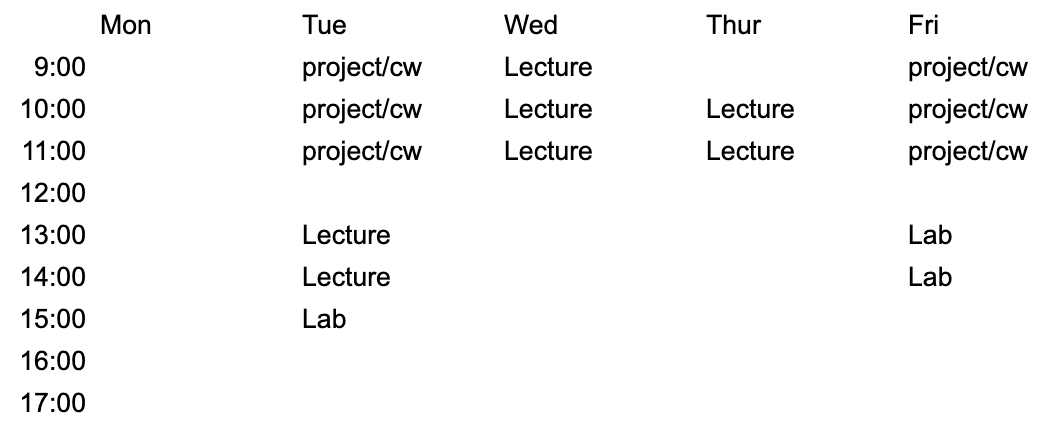
\includegraphics[width=0.8\linewidth]{timetable}
\end{figure}

\end{document}